\subsubsection{Trace equivalence}

The final proof of equivalence will need a number of preliminary lemmata in order to succeed. Most of them describe a series of concrete transformations applied to traces that preserve the semantic meaning of the trace in terms of the effects on the global storage. We start by giving some helpful definitions that will be later used as part of the lemmata.

The first one allows to express that a trace $\tau$ is able to generate a particular storage starting from a given initial state with a storage, lock manager, transactions' stack and program components. It serves the purpose of comparing different traces by establishing a type of trace equivalence. In fact, we obtain important information knowing that two distinct traces $\tau$ and $\tau'$ can generate the same heap under specific circumstances.

\begin{defn}
	(Trace generated).
	A trace $\tau$ \emph{generates} a storage $\underline{h}$ starting from the state $h, \Phi, S, \mathds{P}$ if and only if every action in $\tau$ labels one of consecutive reductions that bring $\mathds{P}$ to $\pskip$ under the \tpl\ operational semantics.
	\begin{align*}
		\pred{tgen}{[], h, \underline{h}, \Phi, S, \mathds{P}}
			\iff&
		h = \underline{h} \land \mathds{P} = \pskip \land \Phi = \emptyset
			\\
		\pred{tgen}{(\alpha, n) : \tau, h, \underline{h}, \Phi, S, \mathds{P}}
			\iff&
		\exists h', \Phi', S', \mathds{P}' \ldotp (h, \Phi, S, \mathds{P}) \xrightarrow{\alpha} (h', \Phi', S', \mathds{P}') \\ &\land \pred{tgen}{\tau, h', \underline{h}, \Phi', S', \mathds{P}'}
	\end{align*}
\end{defn}

In order for the \tpl\ operational semantics to model any kind of two phase locking pattern, we utilize nondeterministic locking of storage cells, as described in Section \ref{sec:opSemCmd2pl}. This comes with the downside of allowing a transaction to lock (and later unlock) any cell it wants. Such phenomenon can happen even if later in the execution the same transaction does not use the locks to access the respective storage cells to read from or write to them. Lock operations performed by a transaction as part of a trace, which are never used to later access the corresponding cell are often and informally referred to as \textit{spurious}. The next two definitions formally describe this behaviour.

\begin{defn}
	(Absent access).
	A cell which is neither read or written to by a given transaction as part of a trace is \emph{absent} and the corresponding predicate is defined as follows:
	\[
		\pred{absent}{\iota, k, \tau}
			\iff
		\lnot \exists v, n \ldotp (\actread{\iota}{k}{v}, n) \in \tau \lor (\actwrite{\iota}{k}{v}, n) \in \tau
	\]
\end{defn}

\begin{defn}
	(Clean trace).
	A trace is \emph{clean} if and only if its transactions do not lock or unlock any absent cell.
	\[
		\pred{clean}{\tau} \iff \forall \iota, k, \kappa, n \ldotp
		\left( (\actlock{\iota}{k}{\kappa}, n) \in \tau \lor (\actunlock{\iota}{k}, n) \in \tau \right)
			\implies
		\lnot \pred{absent}{\iota, k, \tau}
	\]
\end{defn}

\begin{center}
	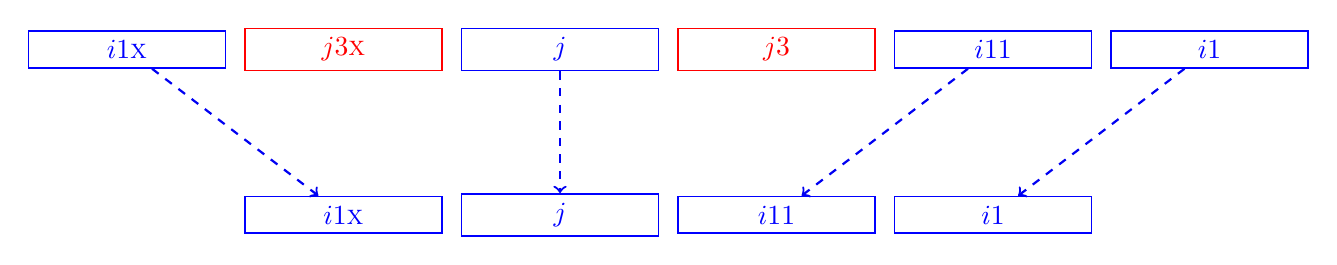
\begin{tikzpicture}[->, semithick]
		\tikzset{
		    tleft/.style= {rectangle, draw=blue, color=blue, minimum width=2.5cm},
		    tright/.style= {rectangle, draw=red, color=red, minimum width=2.5cm},
		    pleft/.style= {above, black!5!blue, thick},
		    pright/.style= {above, black!5!magenta, thick},
		}
		
		\node[tleft] (s1) at (0, 0) {$\actlock{i}{1}{\textsc{x}}$};
		\node[tright] (s2) at (2.75, 0) {$\actlock{j}{3}{\textsc{x}}$};
		\node[tleft] (s3) at (5.5, 0) {$\actid{j}$};
		\node[tright] (s4) at (8.25, 0) {$\actunlock{j}{3}$};
		\node[tleft] (s5) at (11, 0) {$\actwrite{i}{1}{1}$};
		\node[tleft] (s6) at (13.75, 0) {$\actunlock{i}{1}$};
		
		\node[tleft] (s7) at (2.75,-2.1) {$\actlock{i}{1}{\textsc{x}}$};
		\node[tleft] (s8) at (5.5,-2.1) {$\actid{j}$};
		\node[tleft] (s9) at (8.25,-2.1) {$\actwrite{i}{1}{1}$};
		\node[tleft] (s10) at (11,-2.1) {$\actunlock{i}{1}$};
		
		\draw[dashed]
		(s1) edge[pleft] (s7)
		(s3) edge[pleft] (s8)
		(s5) edge[pleft] (s9)
		(s6) edge[pleft] (s10);
	\end{tikzpicture}
	\captionof{figure}{A trace containing spurious locks and its clean equivalent.}
\end{center}

We are able to modify the structure of a trace through the union or the difference with a set of operations, which we formally define as follows.
\begin{defn}
	(Trace difference).
	\[
		\tau' = \tau \setminus S \iff \left( \forall x \ldotp x \not\in S \implies (x \in \tau \iff x \in \tau') \right)
	\]
\end{defn}

\begin{defn}
	(Trace union).
	\begin{gather*}
		\tau' = \tau \cup S \iff \\
		(\forall \alpha, n \ldotp
		(\alpha, n) \in S \implies \left( \lnot \exists \alpha' \ldotp (\alpha', n) \in \tau \right) \\
		\land\ \forall x \ldotp (x \in \tau \lor x \in S) \iff x \in \tau')
	\end{gather*}
\end{defn}

It is now possible to show that any trace $\tau$ that contains a spurious lock (followed by an unlock on the same item) and is able to generate a particular storage $h'$, has a corresponding trace $\tau'$ which contains all of $\tau$'s operations a part from the spurious ones, and $\tau'$ can generate $h'$ starting with the same initial state and program.

\begin{lem}
	(Proof in \ref{lem:lockAbsent}).
	Lock and unlock operations done by a transaction on items which it does not read or write can be removed without affecting the program or the global state.
	\begin{gather*}
		\forall \tau, \tau', h, h', \Phi, S, \mathds{P}, n, n', \iota, k, \kappa, x, y \ldotp
			\\
		\pred{tgen}{\tau, h, h', \Phi, S, \mathds{P}} \land  \pred{absent}{\iota, k, \tau} \land x = (\actlock{\iota}{k}{\kappa}, n) \land y = (\actunlock{\iota}{k}, n') \\ \land x \in \tau \land y \in \tau
		\land \tau' = \tau \setminus \{ x, y \}
			\implies
		\pred{tgen}{\tau', h, h', \Phi, S, \mathds{P}}
	\end{gather*}
\end{lem}

The proof uses another important property of operations inside a trace which is the fact that a lock on an item is not needed for any reductions a part from a read, a write or an unlock action performed by the same transaction on the same item. As we will see later, we leverage this proof in order to \textit{clean} traces from any spurious locks they contain.

\begin{lem}
	(Proof in \ref{lem:alman}).
	\begin{gather*}
		\forall \mathds{P}, \mathds{P}', h, h', \Phi, \Phi', S, S', \alpha, i, k, v, I, \kappa \ldotp \\
		(h, \Phi, S, \mathds{P}) \xrightarrow{\alpha} (h', \Phi', S', \mathds{P}')
			\land
		(\{i\} \uplus I, \kappa) = \Phi(k)
			\land \\
		\alpha \not\in \{ \actread{i}{k}{v}, \actwrite{i}{k}{v}, \actunlock{i}{k} \}
			\implies
		\exists \Phi_m, \Phi_m', I', \kappa', \kappa'' \ldotp \\
		(h, \Phi_m, S, \mathds{P}) \xrightarrow{\alpha} (h', \Phi_m', S, \mathds{P}')
			\land
		\Phi_m = \Phi[k \mapsto (I, \kappa')]
			\land
		\Phi_m' = \Phi'[k \mapsto (I', \kappa'')]
			\land
		\kappa' \leq \textsc{s}
	\end{gather*}
\end{lem}

Once a trace is clean, we can proceed to manipulate it and, under certain cases, swap the order of its operations. Repeating this process, will give us a new trace, syntactically different but semantically equivalent, as observed by its effects on the global heap. This is what we are interested in, given our requirement of simulating a serial trace. Whenever in the following definitions we encounter a term of the shape $\alpha(\iota)$ or $\alpha(\iota, k)$ we actually mean the first projection of their operation-level equivalent, i.e. $op(\iota) \downarrow_1$ and $op(\iota, k) \downarrow_1$ respectively.

\begin{defn}
	(Swapped trace).
	A trace $\tau'$ is the \emph{swapped} version of $\tau$ for some operations $x$ and $y$ if and only if $\tau'$ contains all of $\tau$'s operations in the same exact order a part from the one of $x$ and $y$, which is swapped.
	\begin{gather*}
		\tau' = \pred{swap}{\tau, x, y}
		\iff \\
		\exists \alpha_x, n_x, \alpha_y, n_y \ldotp x = (\alpha_x, n_x) \land y = (\alpha_y, n_y)\ \land \\
		\tau' = \tau \setminus \{(\alpha_x, n_x), (\alpha_y, n_y)\} \cup \{ (\alpha_x, n_y), (\alpha_y, n_x) \}
	\end{gather*}
\end{defn}

The semantically valid swap operations allowed on traces are summarized in the following table, where $\alpha$ and $\alpha'$ label two consecutive operations inside a program trace and the \textit{condition} is the sufficient requirement needed to perform the swap.

\begin{center}
	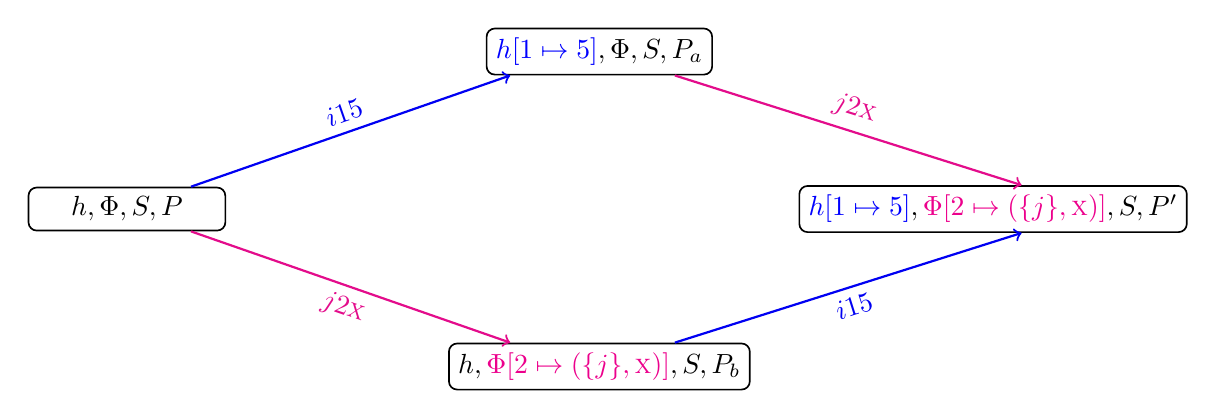
\begin{tikzpicture}[->, semithick]
		\tikzset{
		    tleft/.style= {rectangle, draw=black, color=black, minimum width=2.5cm, rounded corners=3pt},
		    pleft/.style= {above, black!5!blue, thick},
		    pright/.style= {above, black!5!magenta, thick},
		}
		
		\node[tleft] (s1) at (0, 0) {$h, \Phi, S, \mathds{P}$};
		\node[tleft] (s2) at (6, 2) {$\textcolor{blue}{h[1 \mapsto 5]}, \Phi, S, \mathds{P}_a$};
		\node[tleft] (s3) at (6, -2) {$h, \textcolor{magenta}{\Phi[2 \mapsto (\{j\}, \textsc{x})]}, S, \mathds{P}_b$};
		\node[tleft] (s4) at (11, 0) {$\textcolor{blue}{h[1 \mapsto 5]},\textcolor{magenta}{\Phi[2 \mapsto (\{j\}, \textsc{x})]}, S, \mathds{P}'$};
		
		\draw
		(s1) edge[pleft] node[midway, sloped] {$\actwrite{i}{1}{5}$} (s2.195)
		(s1) edge[pright] node[midway, sloped, below] {$\actlock{j}{2}{\textsc{x}}$} (s3.165)
		(s2) edge[pright] node[midway, sloped] {$\actlock{j}{2}{\textsc{x}}$} (s4.40)
		(s3) edge[pleft] node[midway, sloped, below] {$\actwrite{i}{1}{5}$} (s4.320);
	\end{tikzpicture}
	\captionof{figure}{An example of swapping consecutive actions in a program reduction. Note how the end state does not change as a result of the reordering.}
\end{center}

\begin{lem}
	(Swap rules).
	\begin{gather*}
		\forall
			\alpha, \alpha',
			i, j, k, \kappa,
			h, h', h_a,
			\Phi, \Phi', \Phi_a,
			S, S', S_a,
			\mathds{P}, \mathds{P}', \mathds{P}_a
		\ldotp \\
		(h, \Phi, S, \mathds{P})
			\xrightarrow{\alpha}
		(h_a, \Phi_a, S_a, \mathds{P}_a)
			\xrightarrow{\alpha'}
		(h', \Phi', S', \mathds{P}')
			\land
			i \neq j \\
			\land
		\lnot \left( \alpha = \actunlock{i}{k}
			\land
		\alpha' = \actlock{j}{k}{\kappa} \right)
			\land
		\alpha = \alpha(i)
			\land
		\alpha' = \alpha(j) \\
			\implies
		\exists h_b, \Phi_b, S_b, \mathds{P}_b \ldotp
		(h, \Phi, S, \mathds{P})
			\xrightarrow{\alpha'}
		(h_b, \Phi_b, S_b, \mathds{P}_b)
			\xrightarrow{\alpha}
		(h', \Phi', S', \mathds{P}')
	\end{gather*}
	\begin{proof}
	Let's pick arbitrary $\alpha, \alpha' \in \mathsf{Act}, i, j \in \mathsf{Tid}, k \in \mathsf{Key}, \kappa \in \mathsf{Lock}, h, h', h_a \in \mathsf{Storage}$, $\Phi, \Phi', \Phi_a \in \mathsf{LMan}, S, S', S_a \in \mathsf{TState}, \mathds{P}, \mathds{P}', \mathds{P}_a \in \mathsf{Prog}$ and assume that the following holds:
	\begin{gather}
		\label{lem:swapT1}
		(h, \Phi, S, \mathds{P})
			\xrightarrow{\alpha}
		(h_a, \Phi_a, S_a, \mathds{P}_a)
			\xrightarrow{\alpha'}
		(h', \Phi', S', \mathds{P}')
			\land
			i \neq j \\
			\land
		\label{lem:swapT2}
		\lnot \left( \alpha = \actunlock{i}{k}
			\land
		\alpha' = \actlock{j}{k}{\kappa} \right)
			\land
		\alpha = \alpha(i)
			\land
		\alpha' = \alpha(j)
	\end{gather}
	We now proceed in finding $h_b, \Phi_b, S_b, \mathds{P}_b$ by doing a case-by-case analysis on $\alpha$ and $\alpha'$ based on the feasible reductions, i.e. the ones allowed by the \tpl\ operational semantics, they can be part of according to (\ref{lem:swapT1}). From (\ref{lem:swapT2}) we know that neither $\alpha$ nor $\alpha'$ are system transitions $\actprog$. Similarly, we can't have a situation where $\alpha'$ is a lock on a key that has just been unlocked by $\alpha$. Also, since from (\ref{lem:swapT1}) we know that $i \neq j$ meaning that the two actions come from parallel transactions. This implies that, without loss of generality, programs $\mathds{P}, \mathds{P}_a, \mathds{P}'$ have the following shape:
	\[
		\begin{array}{c @{\hspace{15pt}} c @{\hspace{15pt}} c}
			\mathds{P}
				=
			\left( \mathds{T}_i ; \mathds{P}_1 \right)
				\|
			\left( \mathds{T}_j ; \mathds{P}_2 \right)
				\|
			\mathds{P}_3
			&
			\mathds{P}_a
				=
			\left( \mathds{T}_i' ; \mathds{P}_1 \right)
				\|
			\left( \mathds{T}_j ; \mathds{P}_2 \right)
				\|
			\mathds{P}_3
			&
			\mathds{P}'
				=
			\left( \mathds{T}_i' ; \mathds{P}_1 \right)
				\|
			\left( \mathds{T}_j' ; \mathds{P}_2 \right)
				\|
			\mathds{P}_3
		\end{array}
	\]
	Let us also define the new intermediate program, $\dot{\mathds{P}}$, for all the cases we will consider:
	\[
		\dot{\mathds{P}}
			=
		\left( \mathds{T}_i ; \mathds{P}_1 \right)
			\|
		\left( \mathds{T}_j' ; \mathds{P}_2 \right)
			\|
		\mathds{P}_3
	\]
	In the following list we only consider one of the two combinations for each pair as the other one can be trivially found with the appropriate substitutions.
	\begin{enumerate}[label=({\roman*})]
		\item If $\alpha = \actid{i}$ then from the semantic interpretation of $\mathsf{i}$, we obtain that $h_a = h, \Phi_a = \Phi, S_a = S$. It follows that for any action $\alpha'$ performed by $j$ we have the following reduction, from (\ref{lem:swapT1}):
		\[
			(h, \Phi, S, \mathds{P})
				\xrightarrow{\alpha'}
			(h', \Phi', S', \dot{\mathds{P}})
				\xrightarrow{\alpha}
			(h', \Phi', S', \mathds{P}')
		\]
		We can therefore pick $h_b = h', \Phi_b = \Phi', S_b = S'$ and $\mathds{P}_b = \dot{\mathds{P}}$. The same occurs when picking $\alpha' = \actid{j}$ and an arbitrary $\alpha = \alpha(i)$.
		
		\item If $\alpha = \actread{i}{k}{v}$ and $\alpha' = \actread{j}{k'}{v}$ then from the semantic interpretation of $\mathsf{read}$ we know that $h' = h_a = h, \Phi' = \Phi_a = \Phi$. Also, the two $\mathsf{read}$ actions will update transaction-local variables to the values read from the storage so we select $S_b$ to be $S[j \mapsto (s[\pvar{x} \mapsto v], p)]$ where $(s, p) = S(j)$. This implies that we can always reduce in the following way:
		\[
			(h, \Phi, S, \mathds{P})
				\xrightarrow{\alpha'}
			(h, \Phi, S_b, \dot{\mathds{P}})
				\xrightarrow{\alpha}
			(h, \Phi, S', \mathds{P}')
		\]
		We can therefore pick $h_b = h', \Phi_b = \Phi'$ and $\mathds{P}_b = \dot{\mathds{P}}$.
		
		\item If $\alpha = \actread{i}{k}{v}$ and $\alpha' = \actwrite{j}{k'}{v'}$ then from (\ref{lem:swapT1}) it must be the case that $k \neq k'$. This means that given the disjointness of keys, we can always find $h_b = h', \Phi_b = \Phi, S_b = S, \mathds{P}_b = \dot{\mathds{P}}$.
		
		\item If $\alpha = \actwrite{i}{k}{v}$ and $\alpha' = \actwrite{j}{k'}{v'}$ then from (\ref{lem:swapT1}) it must be the case that $k \neq k'$. Now we can always find $h_b = h[k' \mapsto v'], \Phi_b = \Phi, S_b = S, \mathds{P}_b = \dot{\mathds{P}}$.
		
		\item If $\alpha = \actread{i}{k}{v}$ and $\alpha' = \actlock{j}{k'}{\kappa}$ then from (\ref{lem:swapT1}) it must be the case that either $k \neq k'$ or $k = k'$ and $\Phi(k) = (\{i\} \uplus I, \textsc{s})$ and $\kappa = \textsc{s}$. In both cases we can find $h_b = h, \Phi_b = \Phi', S_b = S, \mathds{P}_b = \dot{\mathds{P}}$.
		
		\item If $\alpha = \actwrite{i}{k}{v}$ and $\alpha' = \actlock{j}{k'}{\kappa}$ then from (\ref{lem:swapT1}) it must be the case that $k \neq k'$. Now we can always find $h_b = h, \Phi_b = \Phi', S_b = S, \mathds{P}_b = \dot{\mathds{P}}$.
		
		\item If $\alpha = \actread{i}{k}{v}$ and $\alpha' = \actunlock{j}{k'}$ then from (\ref{lem:swapT1}) it must be the case that either $k \neq k'$ or $k = k'$ and $\Phi(k) = (\{i,j\} \uplus I, \textsc{s})$. In both cases we can find $h_b = h, \Phi_b = \Phi', S_b = S[j \mapsto (s, \pshrink)], \mathds{P}_b = \dot{\mathds{P}}$ for $s = S(j) \downarrow_1$.
		
		\item If $\alpha = \actwrite{i}{k}{v}$ and $\alpha' = \actunlock{j}{k'}$ then from (\ref{lem:swapT1}) it must be the case that $k \neq k'$. Now we can always find $h_b = h, \Phi_b = \Phi', S_b = S', \mathds{P}_b = \dot{\mathds{P}}$.
		
		\item If $\alpha = \actread{i}{k}{v}$ and $\alpha' = \actalloc{j}{n}{l}$ then from (\ref{lem:swapT1}) it must be the case that $k < l \lor l \geq l + n$. Now we can always find $h_b = h', \Phi_b = \Phi', S_b = S[j \mapsto (s[\pvar{x} \mapsto l], p)], \mathds{P}_b = \dot{\mathds{P}}$. Where $\pvar{x}$ is the variable recording the newly allocated address $l$ in transaction $j$ and $(s, p) = S(j)$.
		
		\item If $\alpha = \actwrite{i}{k}{v}$ and $\alpha' = \actalloc{j}{n}{l}$ then from (\ref{lem:swapT1}) it must be the case that $k < l \lor l \geq l + n$. Now we can always find $h_b = h[l \mapsto 0]\ldots[l + n - 1 \mapsto 0], \Phi_b = \Phi', S_b = S[j \mapsto (s[\pvar{x} \mapsto l], p)], \mathds{P}_b = \dot{\mathds{P}}$. Where $\pvar{x}$ is the variable recording the newly allocated address $l$ in transaction $j$ and $(s, p) = S(j)$.
		
		\item If $\alpha = \actlock{i}{k}{\kappa}$ and $\alpha' = \actlock{j}{k'}{\kappa'}$ then from (\ref{lem:swapT1}) it must be the case that either $k \neq k'$ or $k = k'$ and $\kappa = \kappa' = \textsc{s}$. In the first scenario we can find $\Phi_b = \Phi[k' \mapsto (\{j\} \uplus I', \kappa')]$ for $I' = \Phi(k') \downarrow_1$ while in the second one $\Phi_b = \Phi[k \mapsto (\{j\} \uplus I, \textsc{s})]$ for $I = \Phi(k) \downarrow_1$ with $i \not\in I$. In both cases we pick $h_b = h, S_b = S, \mathds{P}_b = \dot{\mathds{P}}$.
		
		\item If $\alpha = \actunlock{i}{k}$ and $\alpha' = \actunlock{j}{k'}$ then from (\ref{lem:swapT1}) it must be the case that either $k \neq k'$ or $k = k'$ and $\Phi(k) = (\{i, j\} \uplus I, \textsc{s})$. In the first scenario we can find $\Phi_b = \Phi[k' \mapsto (I', \kappa'')]$ for $(\{j\} \uplus I', \kappa') = \Phi(k')$, while in the second one $\Phi_b = \Phi[k \mapsto (\{i\} \uplus I, \textsc{s})]$ with $j \not\in I$. In both cases we pick $h_b = h, S_b = S[j \mapsto (s, \pshrink)], \mathds{P}_b = \dot{\mathds{P}}$. for $s = S(j) \downarrow_1$.
		
		\item If $\alpha = \actlock{i}{k}{\kappa}$ and $\alpha' = \actunlock{j}{k'}$ then from (\ref{lem:swapT1}) it must be the case that either $k \neq k'$ and we find $\Phi_b = \Phi[k' \mapsto (I', \kappa'')]$ for $(\{j\} \uplus I', \kappa') = \Phi(k')$ or $k = k'$ and $\Phi(k) = (\{j\} \uplus I, \textsc{s})$ and $\kappa = \textsc{s}$. In the latter case we can find $\Phi_b = \Phi[k \mapsto (I, \textsc{s})]$. In both cases we pick $h_b = h, S_b = S', \mathds{P}_b = \dot{\mathds{P}}$.
		
		\item If $\alpha = \actunlock{i}{k}$ and $\alpha' = \actlock{j}{k'}{\kappa}$ then from (\ref{lem:swapT2}) it must be the case that $k \neq k'$. Now we can always find $h_b = h, \Phi_b = \Phi[k' \mapsto (\{j\} \uplus I, \kappa)], S_b = S, \mathds{P}_b = \dot{\mathds{P}}$ for $(I, \kappa') = \Phi(k'), j \not\in I$ and $\kappa' \leq \textsc{s}$.
		
		\item If $\alpha = \actalloc{i}{n}{l}$ and $\alpha' = \actlock{j}{k}{\kappa}$ then from (\ref{lem:swapT1}) it must be the case that $k < l \lor k \geq l + n$. Now we can always find $h_b = h, \Phi_b = \Phi[k \mapsto (\{j\} \uplus I, \kappa)], S_b = S, \mathds{P}_b = \dot{\mathds{P}}$ for $I = \Phi(k) \downarrow_1$.
		
		\item If $\alpha = \actalloc{i}{n}{l}$ and $\alpha' = \actunlock{j}{k}$ then from (\ref{lem:swapT1}) it must be the case that $k < l \lor k \geq l + n$. Now we can always find $h_b = h, \Phi_b = \Phi[k \mapsto (I, \kappa')], S_b = S[j \mapsto (s, \pshrink)], \mathds{P}_b = \dot{\mathds{P}}$, for $(\{j\} \uplus I, \kappa) = \Phi(k), \kappa' \leq \textsc{s}$ and $s = S(j) \downarrow_1$.
		
		\item If $\alpha = \actalloc{i}{n}{l}$ and $\alpha' = \actalloc{j}{n'}{l'}$ then from (\ref{lem:swapT1}) it must be the case that $\{l, \ldots, l + n - 1\} \cap \{l', \ldots, l' + n' -1 \} \equiv \emptyset$. Now we can always find $h_b = h[l' \mapsto 0]\ldots[l' + n' - 1 \mapsto 0], \Phi_b = \Phi[l' \mapsto (\{j\}, \textsc{x})]\ldots[l' + n' - 1 \mapsto (\{j\}, \textsc{x})], S_b = S[j \mapsto (s[\pvar{x} \mapsto l'], p)], \mathds{P}_b = \dot{\mathds{P}}$ for $(s, p) = S(j)$.
	\end{enumerate}
	All other cases are either ruled out by assumption (\ref{lem:swapT2}) or by the fact that they are unfeasible under the \tpl\ semantics. We provide one of such unfeasible examples for clarity. If $\alpha = \actwrite{i}{k}{v}$ and $\alpha' = \actlock{j}{k}{\textsc{s}}$ for any $v \in \mathsf{Val}$ then in no possible way the original consecutive reduction could have happened. This is because $\alpha$ requires $\Phi(k) = (\{i\}, \textsc{x})$ while $\alpha'$ needs $\Phi_a(k) = (I, \kappa)$ for $\kappa \leq \textsc{s}$. We know that it must be the case that $\Phi_a = \Phi$ since $\alpha$ does not modify the lock manager. It is now clear that such situation could have never occurred.
	\end{proof}
\end{lem}

\begin{defn}
	\label{defn:swappable}
	(Swappable trace actions).
	Two operations as part of a trace  $\tau$ are \emph{swappable} if and only if their indeces are consecutive and for any $\tau$ generated full reduction, there is a point where two consecutive reductions are labelled by them and they are allowed to be swapped.
	\begin{gather*}
		\pred{swappable}{\tau, (\alpha, n), (\alpha', n')} \\
			\iff \\
		n' = n + 1 \land 
		\forall h, \underline{h}, \Phi, S, \mathds{P} \ldotp
		\pred{tgen}{\tau, h, \underline{h}, \Phi, S, \mathds{P}}
			\implies \\
		((\alpha, n) \in \tau
			\land
		(\alpha', n') \in \tau
			\land
		\exists h_1, h_2, h_a, h_b, \Phi_1, \Phi_2, \Phi_a, \Phi_b, S_1, S_2, S_a, S_b, S', \mathds{P}, \mathds{P}_1, \mathds{P}_2, \mathds{P}_a, \mathds{P}_b \ldotp \\
		(h, \Phi, S, \mathds{P})
			\rightarrow^*
		(h_1, \Phi_1, S_1, \mathds{P}_1)
			\xrightarrow{\alpha}
		(h_a, \Phi_a, S_a, \mathds{P}_a)
			\xrightarrow{\alpha'}
		(h_2, \Phi_2, S_2, \mathds{P}_2)
			\rightarrow^*
		(\underline{h}, \emptyset, S', \pskip) \\
			\land\
		(h_1, \Phi_1, S_1, \mathds{P}_1)
			\xrightarrow{\alpha}
		(h_b, \Phi_b, S_b, \mathds{P}_b)
			\xrightarrow{\alpha'}
		(h_2, \Phi_2, S_2, \mathds{P}_2))
	\end{gather*}
\end{defn}

\begin{lem}
	(Trace swap equivalence).
	\begin{gather*}
		\forall h, \underline{h}, \Phi, S, \mathds{P}, \tau, \tau', x, y \ldotp \\
		\pred{tgen}{\tau, h, \underline{h}, \Phi, S, \mathds{P}}
			\land
		\pred{swappable}{\tau, x, y}
			\land
		\tau' = \pred{swap}{\tau, x, y}
			\implies
		\pred{tgen}{h, \underline{h}, \Phi, S, \mathds{P}}
	\end{gather*}
	\begin{proof}
	Let's pick arbitrary $h, \underline{h} \in \mathsf{Storage}, \Phi \in \mathsf{LMan}, S \in \mathsf{TState}, \mathds{P} \in \mathsf{Prog}, \tau, \tau' \in [\mathsf{Act} \times \mathds{N}], x, y \in \mathsf{Act} \times \mathds{N}$. We now assume that the following holds:
	\[
		\pred{tgen}{\tau, h, \underline{h}, \Phi, S, \mathds{P}}
			\land
		\pred{swappable}{\tau, x, y}
			\land
		\tau' = \pred{swap}{\tau, x, y}
	\]
	The above means that we can generate the $\underline{h}$ storage from $\tau$ starting with state $(h, \Phi, S, \mathds{P})$ and there are two operations $x = (\alpha, n), y = (\alpha', n + 1)$ which are $\mathsf{swappable}$ as defined in Definition \ref{defn:swappable}. We also know that another trace, $\tau'$, is equivalent to $\tau$ with operations $x$ and $y$ swapped. It is required to show that $\tau'$ can also generate $\underline{h}$ starting from $(h, \Phi, S, \mathds{P})$.
	
	From the definition of $\mathsf{swappable}$, we know that the following must hold, where the non-bound variables are assumed to be existentially quantified for conciseness:
	\begin{gather}
		\label{lem:tswap1}
		(h, \Phi, S, \mathds{P})
			\rightarrow^*
		(h_1, \Phi_1, S_1, \mathds{P}_1)
			\xrightarrow{\alpha}
		(h_a, \Phi_a, S_a, \mathds{P}_a) \\
		\label{lem:tswap2}
			\xrightarrow{\alpha'}
		(h_2, \Phi_2, S_2, \mathds{P}_2)
			\rightarrow^*
		(\underline{h}, \emptyset, S', \pskip) \\
		\label{lem:tswap3}
			\land\
		(h_1, \Phi_1, S_1, \mathds{P}_1)
			\xrightarrow{\alpha}
		(h_b, \Phi_b, S_b, \mathds{P}_b)
			\xrightarrow{\alpha'}
		(h_2, \Phi_2, S_2, \mathds{P}_2)
	\end{gather}
	From (\ref{lem:tswap1}) and the definition of $\mathsf{swap}$ we obtain that, following $\tau'$ for $n - 1$ steps we can reduce $(h, \Phi, S, \mathds{P}) \rightarrow^* (h_1, \Phi_1, S_1, \mathds{P}_1)$. Next, we know that $\alpha$ and $\alpha'$ are swapped in $\tau'$, meaning that from (\ref{lem:tswap3}) we can reduce $(h_1, \Phi_1, S_1, \mathds{P}_1) \xrightarrow{\alpha} (h_b, \Phi_b, S_b, \mathds{P}_b) \xrightarrow{\alpha'} (h_2, \Phi_2, S_2, \mathds{P}_2)$ and we reach step $n+2$. From then on $\tau$ and $\tau'$ are equivalent, therefore the from (\ref{lem:tswap2}) we reduce until $\pskip$ to a state whose storage component is $\underline{h}$.
	\end{proof}
\end{lem}